\section{The \acs{EsPy} \acs{GUI}}
\begin{figure}
    \centering
    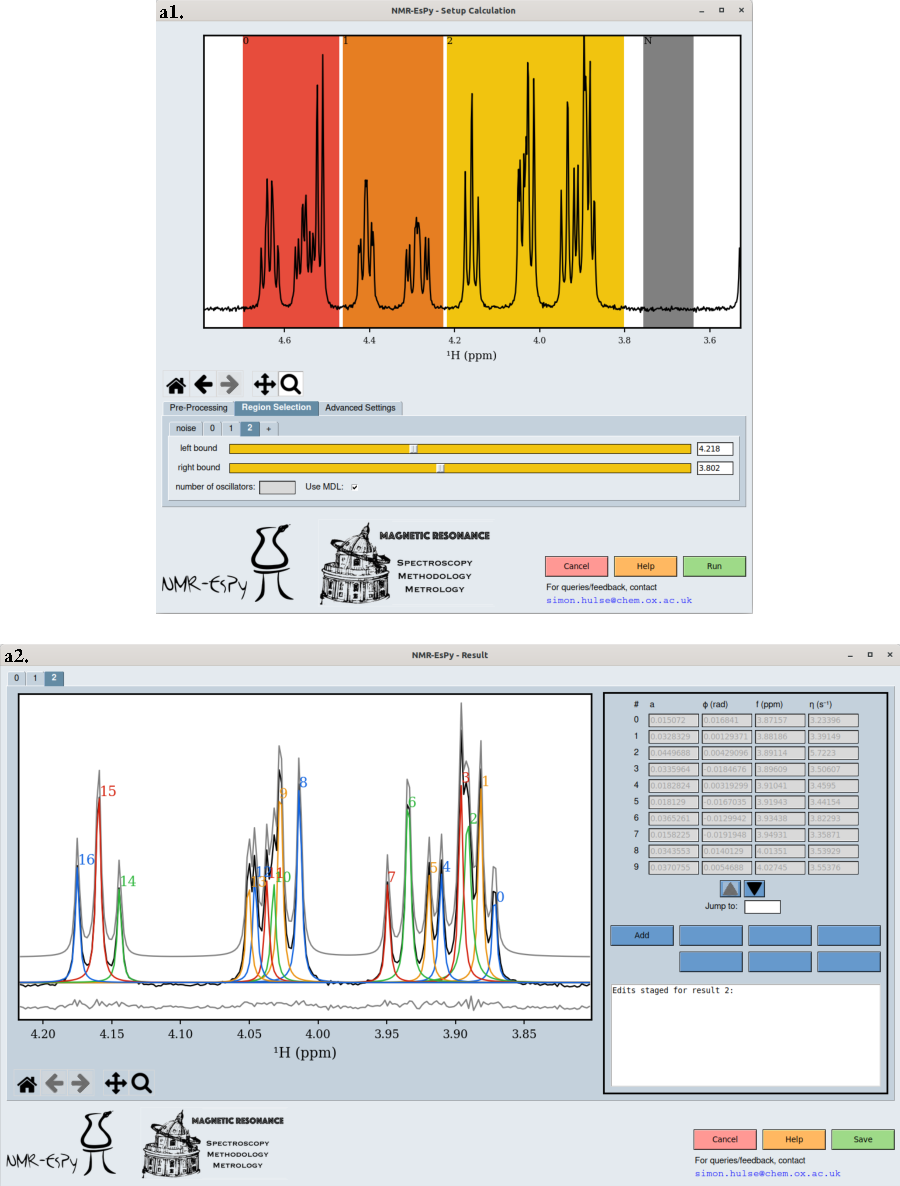
\includegraphics{gui/gui_1d.pdf}
    \caption[
        The appearence of the \acs{EsPy} \acs{GUI} for \acs{1D} and \acs{2DJ}
        estimation.
    ]{
        Screenshots of windows that form part of the \ac{EsPy} \ac{GUI} for
        \ac{1D} estimation (\textbf{a.}) and \ac{2DJ} estimation (\textbf{b.}).
        For both data types, the windows used to setup the estimation routine
        (\textbf{1.}) and inspect the result (\textbf{2.}) are shown.
        (Continues on the next page)
    }
    \label{fig:gui}
\end{figure}
\begin{figure}%
    \ContinuedFloat
    \centering
    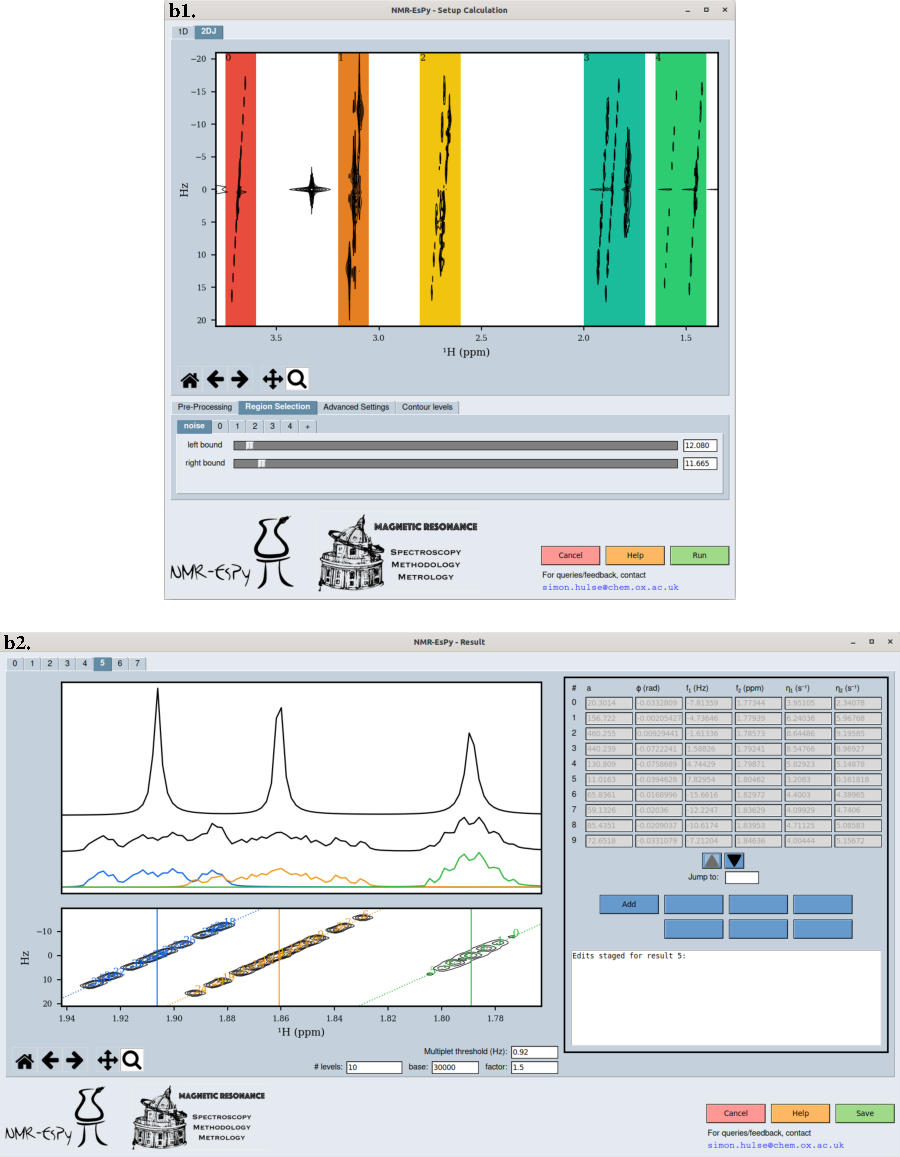
\includegraphics{gui/gui_2dj.pdf}
    \caption*{Continuation of \textbf{\cref{fig:gui}}.}
\end{figure}
Along with the \ac{EsPy} \ac{API}, an accompanying \ac{GUI}, created using
\textsc{Python}'s in-built \textsc{Tkinter} toolkit~\cite{tkinter}, ships with
the package. The \ac{GUI} can be accessed either via the command line, or within
\textsc{Bruker}'s \textsc{TopSpin} software to provide a more seamless workflow
in analysing \ac{NMR} data acquired on \textsc{Bruker} spectrometers.
At the time of writing, the \ac{GUI} only supports conventional \ac{1D}
and \ac{2DJ} datasets. Screenshots of the \acp{GUI} are provided in
\cref{fig:gui}.
The \ac{GUI} comprises two primary windows; the first enables the estimation
routine to be set up (Figures \ref{fig:gui}.a1 and \ref{fig:gui}.b1), while the
second is for inspecting the result and exporting information about it to the
desired format(s) (Figures \ref{fig:gui}.a2 and \ref{fig:gui}.b2).

The set-up window allows the following actions to be carried out:
\begin{itemize}
    \item The \emph{Pre-Processing} tab facilitates phase correction,
        application of exponential line-broadening\footnote{
            Exponential line-broadening is the only type of apodisation which
            is supported in \ac{EsPy}; use of any other window function
            would render the model used to fit the data incompatible.
            Line-broadening should only be applied in
            situations where the \ac{FID} is truncated, such that sinc wiggles
            are visible in the spectrum, as these will have an unwanted
            influence on filtered sub-\acp{FID} generated.
        }, and baseline correction. If the imported data have already been
        processed by some other software such as \textsc{TopSpin}\footnote{
            For \ac{1D} datasets, it is possible to import raw \ac{FID} data
            (\texttt{fid}) or processed spectral data (\texttt{1r}). If
            pre-processed data is imported, \ac{EsPy} performs \ac{IFT} and
            truncates the conjugate-symmetric signal generated in half to
            recover the \ac{FID}. For \ac{2DJ} data, it is necessary to import
            \ac{2DJ} data as a raw \ac{FID} (\texttt{ser}).
        }, this step can be skipped.
    \item The regions of interest and the noise region are
        defined with the \emph{Region Selection} tab. Examples of the
        appearance of the \ac{GUI} after a number of regions have been defined
        by the user are given in Figures \ref{fig:gui}.a1 and \ref{fig:gui}.b1;
        regions of interest are denoted by various colours, while the noise region
        is grey.
    \item \emph{Additional Settings} allows features related of the estimation
        routine to be customised, including whether to approximate the Hessian
        matrix or compute its exact form, whether to predict the model order
        using the \ac{MDL} or to manually specify a value, and setting a
        threshold for the maximum number of iterations allowed before the
        \ac{NLP} routine terminates.
\end{itemize}

The result window features a figure depicting the outcome of the
estimation routine with a table of all the estimated parameters.
% For any
% features in the result which the user deems to be erroneous, there is scope for
% some basic edits to be made to be. Oscillators can be \emph{added} to the
% result if a particular signal has been missed by the routine; they can be
% \emph{removed} if they are deemed spurious; multiple oscillators can be
% \emph{merged} if a particular signal is deemed to be over-fit; and a single
% oscillator can be \emph{split} if more than one signal is deemed to be
% under-fit. If any edits are requested by the user, the updated parameter set is
% subjected to \ac{NLP} in order to reduce the bias in the result, and ensure
% good agreement between the model and data is maintained. The ability to edit
% the result can lead to better outcomes, since the user is able to guide the
% optimiser using their expertise.
The final stage in using the \ac{GUI} involves specifying the formats to output
the result to. Figures and parameter tables summarising the result can be
exported to various formats. Simulated signals constructed using the
parameter estimate, such as the pure shift spectrum and individual multiplets
structures produced by \ac{CUPID}, may also be created.
